\section{Dokumentation}
\subsection{Forklar hvad arv er}
Et af de vigtigste elementer i objektorienteret programmering er nedarvning, men hvad betyder nedarvning? At arve betyder i bund og grund at noget med en materiel værdi overdrages til noget eller nogle efterkommere. I programmerings verden ville man hellere definere arv som en eller flere egenskaber der overføres fra en generation til en anden generation, også sagt på en anden måde, at en klasse der får overført egenskaber fra en anden klasse. Den klasse der nedarves fra kaldes for en Superklasse (parent), hvor klassen der nedarver eller får egenskaber fra en Superklasse, kaldes for en Subklasse (child). (Kressner, Marts 2014)
Ved benyttelse af denne proces vil oplysningerne om de forskellige klasser ende op i en hierarkisk rækkefølge. 
På figuren ses forskellige eksempler på typer af nedarvning der findes, men dog skal man være opmærksom på, at Java ikke understøtter flere nedarvninger. I Java kan en klasse kun have én Superklasse, dvs. at hver klasse kun kan nedarve fra én klasse. (Kressner, Marts 2014)
\begin{figure}[h]\label{fig:types_of_inheritance.jpg} 
    \advance\leftskip-3cm
    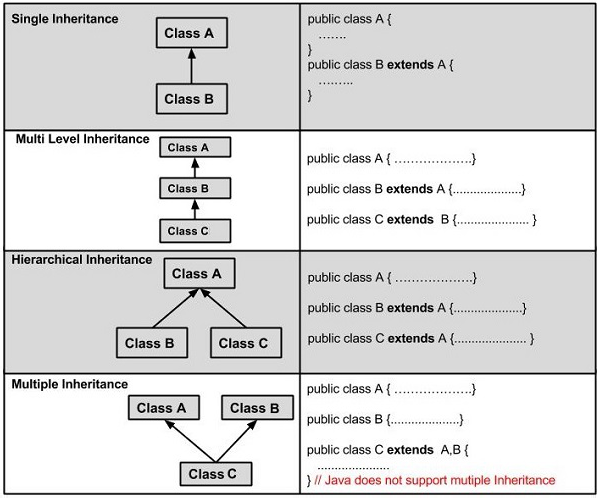
\includegraphics[width=6cm]{fig/types_of_inheritance.jpg}
    \caption{eksempel på typer af arv}
\end{figure}
\subsection{Forklar hvad abtract betyder}
Den abstrakte klasse kører ingen metoder og indeholder kun attributter. Klassen bruges som en slags ”over”-klasse, hvor andre klasser nedarver attributterne. Det anvendes i situation, hvor man f.eks har to klasser, der har mange af de samme attributter. Så ville alle de attributter som de har filfælles stå i den abstrakte klasse.
Hvis man f.eks har klasserne lærer og elev, kunne den abstrakte klasse til disse, hedde ”personer”, da både lærer og elever har en fødselsdato, køn, navn osv.

\subsection{Fortæl hvad det hedder hvis alle fieldklasserne har en landOnField metode der gør noget forskelligt}

% IOException: Sentence length out of bounds.
Hvis alle fieldklasserne gør brug af den samme landOnField metode, er det fordi denne metode er en super metode. En super metode er nedarvet til de forskellige subklasser fra super klassen, dette gør at alle klasserne kan gøre brug af samme metode. Eksempeltvis, hvis vi har en masse dyr som klasser, kat, hund, kanin etc. så kan de alle nedarve super metoden eat() fra 
superklassen som hedder SurvivalRequirements, eftersom disse er metoder alle dyrene får brug for, så vil det give mening at lave det til en superklasse med supermetoder
, så der holdes lav kobling og høj kohæsion, samt undgås kopiring af kode og høj mulighed for genbrug.

\subsection{Dokumentation for test med screenshots}
    \subsection{JUnit test}
        JUnit test er en autonomisreret testmetode. Her skriver/koder man selv en test, som tester java kode. Oftest opbygger man JUnit test ud fra Java klasser.
        Der er mange måder hvorpå man kan bruge JUnit testen. Man kan både skrive testen inden, man kan skrive den efter, man kan lave den på baggrund af indsigt i koden eller uden nogen form til kendskab af programkoden. Det to sidst nævnte kaldes Black- og Whitebox test.
        Her er et eksempel på et stykke udført JUnit test fra vores spil:
            \begin{figure}[h]\label{fig:JUnitTest} %FIGUR 7???
                \advance\leftskip-3cm
                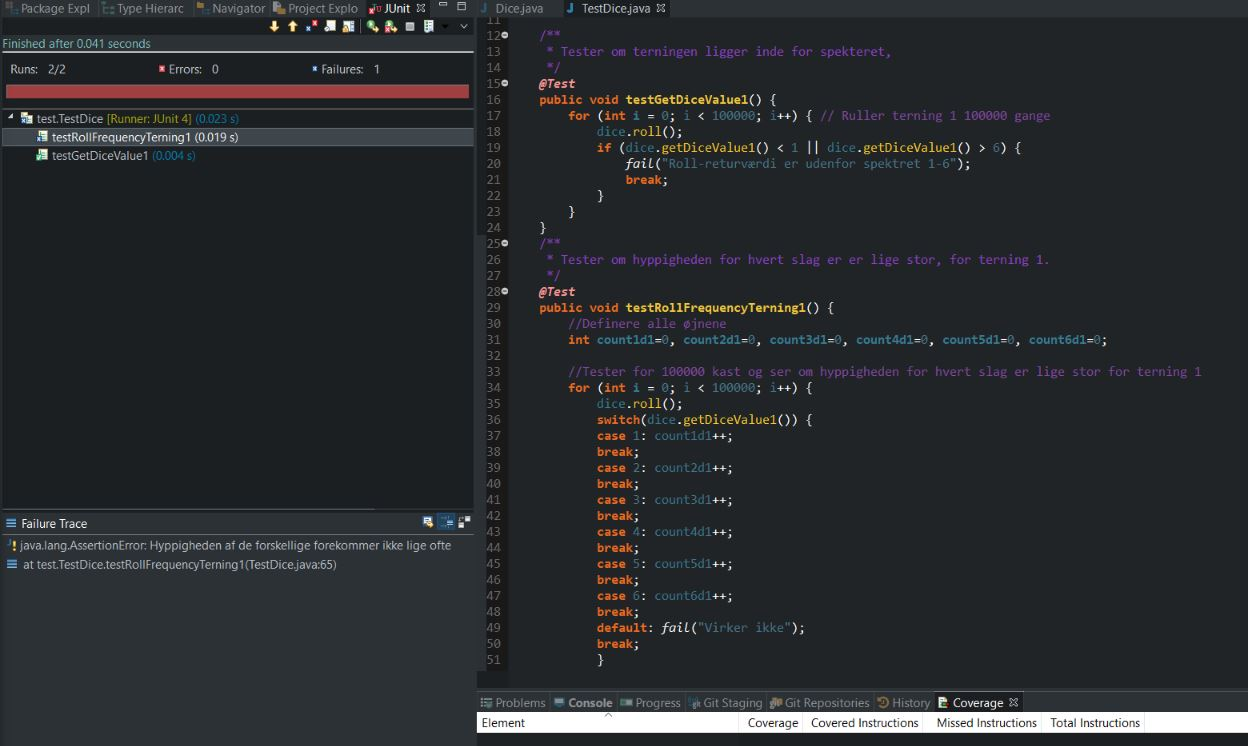
\includegraphics[width=20cm]{fig/JUnitTestDice.jpg}
                \caption{JUnit test udført i Eclipse den 23/11-2017}
            \end{figure}
        Det ser på Figur \ref{fig:JUnitTest} at koden ikke bestod testen, hvor vi også får vist den rette, selv skrevet, fejl besked.

    \subsection{Positiv negativ test}
        Denne test bruges for at teste om systemet kan håndterer 'ugyldige' input, dette kan både være negative som positive værdier, såvel som bogstaver og andre tegn. Denne test forbindes oftest med en eller flere ækvivalensklasse test.
    \subsection{Black- og Whitebox test}
        \textbf{Blackbox test}: Her har du intet kendskab til koden, ud over hvad denne skal kunne gøre. Det er derfor --lige til højre benet-- at teste det faktiske output, mod det forventede output og at teste ækvivalensklasserne.
        \textbf{Whitebox test}: Her opstiller man tests på baggrund af koden og dens opbygning. Man vil med disse tests teste hele koden, altså alle instruktioner, forgreninger og stier, som koden kan blive udført i. Dette er ikke altid muligt med \textit{BlackBox testen} , da man her ikke har et indblik i koden.

\subsection{Dokumentation for overholdt GRASP}

\subsection{Vejledning til import af Git Repository til eclipse}
Man skal i første omgang have et URL af det pågældende repository, som du kopierer.
Derefter åbner du eclipse og åbner menuen 
Window $\Rightarrow$ View $\Rightarrow$ søg på "git" $\Rightarrow$ git repositories.
Derefter har du vinduet "Git Repositories", hvor der er en knap; "Clone a git repository and add to this view".
Ikonet er mappen i midten med en blå pil på, her trykker du.
Hvis du huskede at kopiere URL'et trykker du nu "Next", hvorefter at alle branches bliver loaded. Når den har loaded trykker du next igen.
Nu kommer du til det sidste vindue, hvor du trykker "Finish, og nu har du importeret(clonet) git repositoriet.
